\title{Computational Neurophysiology - Assignment 4}
\author{Ryan Spangler}
\date{\today}

\documentclass[12pt]{article}

\usepackage{commath}
\usepackage{graphicx}

\setcounter{secnumdepth}{0}

\begin{document}
\maketitle

\section{Integrate and Fire - Analysis}

The basic integrate and fire equation can be solved directly for voltage.  In its original form

$$ \tau_m\od{V(t)}{t}=(E_{leak}-V(t))+R_mI $$

the integrate and fire model has a constant resistance and a constant current.  If the current varies with time, as in

$$ \tau_m\od{V(t)}{t}=(E_{leak}-V(t))+R_mI(t) $$

it can still be integrated, but the function $I(t)$ must be specified.  For this example we will choose the simple function $I(t)=cos(t)$ and thus

$$ \tau_m\od{V(t)}{t}=(E_{leak}-V(t))+R_mcos(t) $$

As this is a linear system, to tackle this problem we can separate the equation into its homogenous and nonhomogenous components $\alpha$ and $\beta$, 

$$ \od{V(t)}{t}=\alpha(t)V(t)+\beta(t) $$

Thus, the component relevant only to V(t) can be written

$$ \od{V(t)}{t}=\frac{-1}{\tau_m}V(t) $$

with a ready solution of this homogenous part of the equation:

$$ V_H(t)=e^{\frac{-t}{ \tau_m}} $$

The nonhomogenous component focusing on the non-V(t) terms would look something like this:

$$ \od{V(t)}{t}=\frac{E_{leak}+R_mcos(t)}{\tau_m} $$

Taking the antiderivative of this yields

$$ V_N(t)=\frac{E_{leak}t+R_msin(t)}{\tau_m} $$

which, adding together the homogenous and nonhomogenous solutions, yields the ultimate solution

$$ V(t)=V_H(t)+V_N(t)=e^{\frac{-t}{\tau_m}}+\frac{E_{leak}t+R_msin(t)}{\tau_m} $$

which can be checked by differentiating and receiving the original equation back again.

\section{Integrate and Fire - Simulation}

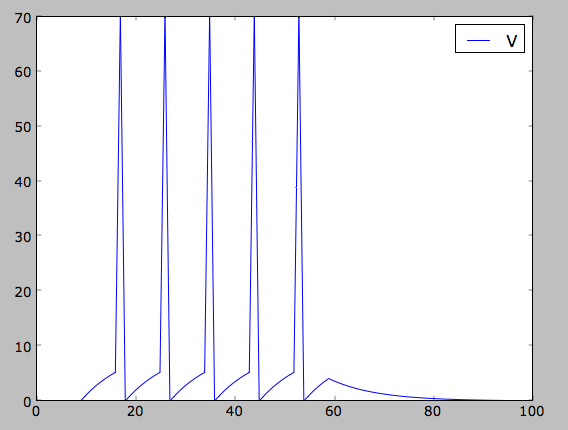
\includegraphics[scale=0.71]{integratefirespikes.png}

\section{Spike-Response Models - Analysis}



\section{Poisson Spikes}



\end{document} 
